\title{PS7 Solutions}

%TEMPLATE HEADER
%This is the homework solution template
\documentclass[11pt]{article}

%AMS-TeX packages
\usepackage{amssymb, amsmath, amsthm} 
\usepackage[margin=.75in]{geometry}
\usepackage{graphicx}
\usepackage{caption}
\usepackage{subcaption}
\usepackage{bm} % bold math
\usepackage{listings}
\usepackage{color} %red, green, blue, yellow, cyan, magenta, black, white
\definecolor{mygreen}{RGB}{28,172,0} % color values Red, Green, Blue
\definecolor{mylilas}{RGB}{170,55,241}

%Redefining sections as problems
\makeatletter
\newenvironment{problem}{\@startsection
       {section}
       {1}
       {-.2em}
       {-3.5ex plus -1ex minus -.2ex}
       {0.2ex plus .2ex}
       {\pagebreak[3]%forces pagebreak when space is small; use \eject for better results
       \Large\sc\noindent{Problem }}\\}
\makeatother

%Fancy-header package to modify header/page numbering 
\usepackage{fancyhdr}
\pagestyle{fancy}
\lhead{\textbf{Ge/ESE 118}} %name of the course
\chead{\textbf{}} %topic of the homework set
\rhead{\textbf{Solution 7}} %number of the homework set
\lfoot{}
\cfoot{}
\rfoot{\thepage}

%Include frequently used commands used for equations
%Fractions
\newcommand\fr[2]{\frac{#1}{#2}} %Regular fraction

%Braces, Brackets, Parentheses, etc.
\newcommand\brcs[1]{\{#1\}} %Braces
\newcommand\brckts[1]{\left[#1\right]} %Brackets
\newcommand\lr[1]{\left(#1\right)} %Parentheses
\newcommand\abs[1]{\Big\lvert#1\Big\rvert} %Absolute value
\newcommand\ltwo[1]{\lVert#1\rVert_2} %L2-norm
\newcommand\linf[1]{\lVert#1\rVert_\infty} %L2-norm

%Linear algebra
\newcommand\tr[1]{\text{tr}\left( \mathbf{#1}\right)} %Trace
\renewcommand\det[1]{\text{det}\left( \mathbf{#1}\right)} %Determinant

%Trigonometric & special functions
\newcommand\sinb[1]{\, \sin\left(#1\right)} %Sine with parentheses: sin(x)
\newcommand\cosb[1]{\, \cos\left(#1\right)} %Cosine with parentheses: cos(x)
\newcommand\tanb[1]{\, \tan\left(#1\right)} %Tangent with parentheses: tan(x)
\newcommand\cotb[1]{\, \cot\left(#1\right)} %Cotangent with parentheses: cot(x)
\newcommand\sinc[1]{\, \text{sinc}\left(#1\right)} %Sinc function: sinc = sin(x)/x

%Calculus
\renewcommand\d[1]{\, \text{d}#1} %Differential for integrals
\newcommand\der[2]{\frac{\text{d}#1}{\text{d}#2}} %Ordinary derivate first order
\newcommand\dder[2]{\frac{\text{d}^2#1}{\text{d}#2^2}} %Ordinary derivate second order
\newcommand\od[3]{\frac{\text{d}^{#3}#1}{\text{d}#2^{#3}}} %Ordinary derivate any order
\newcommand\pder[2]{\frac{\partial#1}{\partial#2}} %Partial derivate first order
\newcommand\pdder[2]{\frac{\partial^2#1}{\partial#2^2}} %Partial derivate second order
\newcommand\pd[3]{\frac{\partial^{#3}#1}{\partial#2^{#3}}} %Partial derivative any order

%Fourier transform
\newcommand\ft[1]{\hat{#1}} %Fourier coefficient

%Probability theory, Statistics
\newcommand\ex[1]{\mathbb{E}\left[#1\right]} %Expectation
\newcommand\pr[1]{\mathbb{P}\left(#1\right)} %Probability
\newcommand\Var[1]{\text{Var}\left(#1\right)} %Variance
\newcommand\Cov[1]{\text{Cov}\left(#1\right)} %Covariance
\newcommand\one{\mathbf{1}} %Unity

%Miscellaneous 
\renewcommand\mod{\text{mod}} %Modulo

%CONTENTS OF THE HW SET SOLUTION BEGIN HERE
\begin{document}
\lstset{language=Matlab,%
	  %basicstyle=\color{red},
  breaklines=true,%
  morekeywords={matlab2tikz},
  keywordstyle=\color{blue},%
  morekeywords=[2]{1}, keywordstyle=[2]{\color{black}},
  identifierstyle=\color{black},%}
  stringstyle=\color{mylilas},
  commentstyle=\color{mygreen},%
  showstringspaces=false,%without this there will be a symbol in the places where there is a space
  numbers=left,%
  numberstyle={\tiny \color{black}},% size of the numbers
  numbersep=9pt, % this defines how far the numbers are from the text
  emph=[1]{for,end,break},emphstyle=[1]\color{red}, %some words to emphasise
													  %emph=[2]{word1,word2}, emphstyle=[2]{style},    
}



\subsection*{Problem 1 (graded by Dunzhu) 20 points}

\subsubsection*{(a)- 5 points}
if $[U,S,V]=svd(G)$, so $G=U*S*V^{T}$, thus $G^{-1}_g=V*S^{-}*U^{T}$. Note $S^{-}_{i,i} = 1/S_{i,i}$ for $S_{i,i}\neq 0$, and $S^{-}_{i,i} =0 $ for $S_{i,i} = 0$. The result is
\begin{verbatim}
R1 =
    0.2839    0.4645    0.1484    0.1032
   -0.0194   -0.1226    0.0581    0.0839
R2 =
    0.2769    0.2154    0.3231    0.1846
   -0.3590    0.4615   -0.9744    0.8718
R3 =
    2.2194   12.7226   -5.6581   -8.2839
   -0.0194   -0.1226    0.0581    0.0839
R4 =
    0.0250    0.0250    0.0250    0.0250
    0.0750    0.0750    0.0750    0.0750
\end{verbatim}

\subsubsection*{(b)- 5 points}
$ G^{-1}_{LLS} = inv(G^{T}*G)*G^{T}$. But if $\det{G^{T}*G}=0$, then the least square problem will have infinitely many solutions that gives the same minimized error, which means $G^{-1}_{LLS}$ is not well defined in this case. 
\begin{verbatim}
L1 =
    0.2839    0.4645    0.1484    0.1032
   -0.0194   -0.1226    0.0581    0.0839
L2 =
    0.2769    0.2154    0.3231    0.1846
   -0.3590    0.4615   -0.9744    0.8718
L3 =
    2.2194   12.7226   -5.6581   -8.2839
   -0.0194   -0.1226    0.0581    0.0839
L4 =
   Inf   Inf   Inf   Inf
   Inf   Inf   Inf   Inf

\end{verbatim}
\lstinputlisting{hw7p1.m}

\subsubsection*{(c)- 5 points}
When least square inverse is unique, $\det{G^{T}*G}\neq 0$, $G^{-1}_{LLS}$ is the same as general inverse, because
\begin{eqnarray*}
G & = & U*S*V^T \\
G^T & = & V*S^T*U^T \\
G^T*G & = & V*(S^T*S)*V^T \\
(G^T*G)^{-1} & = & V*(S^T*S)^{-1}*V^T \\
(G^T*G)^{-1}*G^T & =& V*(S^T*S)^{-1}*S^T*U^T \\
 &=& V*S^{-}*U^T \\
 &=& G^{-1}_g
\end{eqnarray*}
which is the same as generalized inverse. Note in the above derivation, $U$,$V$ is square orthgonal matrix, where $S$, $S^-$ is diagnoal but not square matrix, and $S^T*S$ has inverse. 

When $\det{G^{T}*G} = 0$ , $G^{-1}_{LLS}$ is not well defined,  and general inverse gives the solution that satisfies least square problem and at the same time minimizes the L2 norm of the model. 

\subsubsection*{(d)- 5 points}
Note that $G^{-1}_g d $ gives the estimation of intercept and slope of the 4 points least square problem, whose $X$ is given by second column of $G$. This explains why  $G_{1g}^{-1}$ has the same second row as $G_{3g}^{-1}$, because $X$ in $G_3$ is just a shift of $X$ in $G_1$. 

For $G_1,G_2,G_3$, the two columns are linearly independent, so they have full column rank, then
\begin{eqnarray*}
G^{-1}_g*G & = & V*S^-*U^T * U*S*V^T \\
      & = & V* S^- * S * V^T \\
      & = & V*V^T\\
      & = & I      
\end{eqnarray*}
So the 1st row of $G^{-1}_g$ dot product with 1st column of $G$ will be 1, the 2nd row of $G^{-1}_g$ dot product with 2nd column of $G$ will be 1, and the 1st row of $G^{-1}_g$ dot product with 2nd column of $G$ will be 0, the 2nd row of $G^{-1}_g$ dot product with 1st column of $G$ will be 0. This explains roughly, for example, the relative higher amplitude of the first row of $G_3^-$ compared with the 2nd row of $G_3^-$. However, we must be careful about such amplitude comparison, because for example the 2nd row of $G_1^{-1}$ and the 2nd row of $G_3^{-1}$ is the same, although amplitude in $G_1$ and $G_3$ is quite different.

For $G_4$, whose rank is 1,  note that the least square solution will require $m_1 + 3 m_2 = const$. This is a line in $m_1 ~ m_2$ plane. The L2 norm of the model, will corresponding to a line segment from origin to this line, which got minimized when it's perpendicular to this line, or $m_1 / m_2 = 1 / 3$. This explains why $G_4^{-1}$, also a rank 1 matrix, has two rows whose amplitude ratio is 1/3. 


\subsection*{Problem 2 (graded by Stephen) 25 points}

\subsubsection*{(a)- 5 points}
Looking at the SVDs of the G matrices from problem 1, we see a couple inverses that would potentially benefit from a truncated SVD.  Truncation is a useful strategy when there is a large disparity between sizes of singular values.  We don't care about the absolute value of the singular values (unless they are close to machine precision $(~10^-16)$), we only care about the relative size of the singular values to one another.  The first 3 G matrices each have two singular values, so we can take the ratio of these two values to see which matrices might require truncation.  G4 only has 1 nonzero singular value, so it is effictively already truncated.  If we look at the ratios of singular values $\frac{s_2}{s_1}$ we get:

\begin{equation}
G1: \frac{s_2}{s_1}= 0.2393
\end{equation}

\begin{equation}
G2: \frac{s_2}{s_1}= 0.3469
\end{equation}

\begin{equation}
G3: \frac{s_2}{s_1}= 3.000*10^{-4}
\end{equation}

G3 has the smallest ratio by several orders of magnitude, so it is out best candidate for truncation.
G1 has a smaller ratio than G2, so it would be our second most amenable matrix for truncation.

Truncation has the advantage of removing errors potentially caused by small singular values; thus, not allowing these errors to propagate through the rest of our calculations.  However, the disadvantage here is that we are removing information and often the smallest singular values also contain the most information.  We want to use truncation in order to keep the most amount of information that isn't dominated by errors or noise.

\subsubsection*{(b)- 5 points}
We select G3 as the most amenable to a truncated SVD.  The recalculation yields:

\begin{equation}
G3_{GeneralizedInverseTruncated} = 
\begin{pmatrix}
0.0000 & 0.0000 & 0.0000 & 0.0000\\
0.0024 & 0.0023 & 0.0025 & 0.0025\\
\end{pmatrix}
\end{equation}

\subsubsection*{(c)- 5 points}
The second most amenable matrix is G1.  The recalculation 

\begin{equation}
G3_{GeneralizedInverseTruncated} = 
\begin{pmatrix}
0.0031 & -0.0078 & 0.0114 & 0.0141\\
0.0216 & -0.0537 & 0.0780 & 0.0969\\
\end{pmatrix}
\end{equation}

\lstinputlisting{hw7p2.m}

\subsubsection*{(d)- 5 points}
We calculate the generalized inverse model solutions using both the original SVD and the truncated versions for both G1 and G3 for each of the datasets $d_1$ and $d_2$.  The plots are attached below.  Here are the solutions:

\begin{verbatim}
m1d1 =

   10.5226
   -0.0129


m1d2 =

   10.4652
   -0.2658


m3d1 =

   11.8129
   -0.0129


m3d2 =

   37.0458
   -0.2658


mt1d1 =

    0.2171
    1.4893


mt1d2 =

    0.1798
    1.2335


mt3d1 =

    0.0010
    0.1031


mt3d2 =

    0.0010
    0.0979
\end{verbatim}


\begin{figure}
\begin{center}
  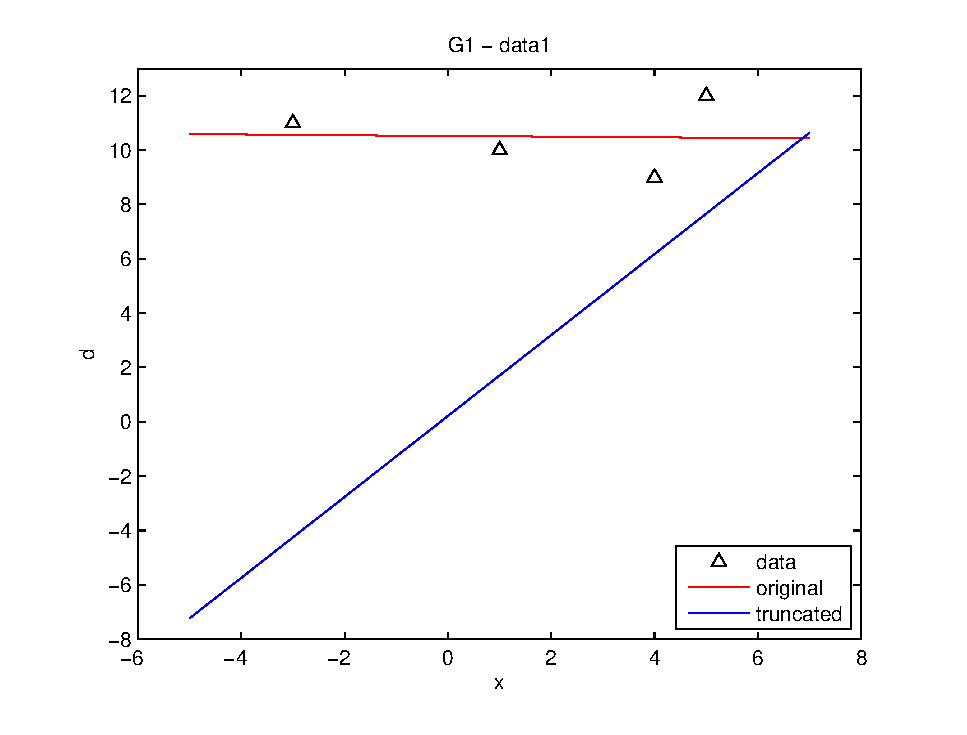
\includegraphics[width=12cm]{p2fig1.eps}
  \end{center}
\end{figure}
\begin{figure}
\begin{center}
  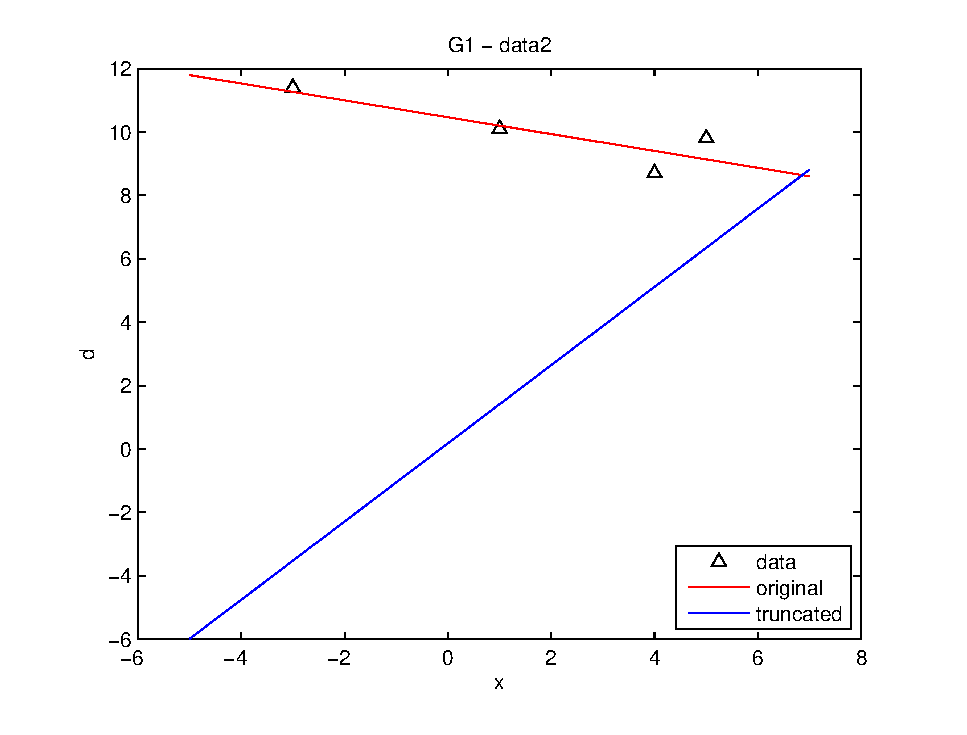
\includegraphics[width=12cm]{p2fig2.eps}
  \end{center}
\end{figure}
\begin{figure}
\begin{center}
  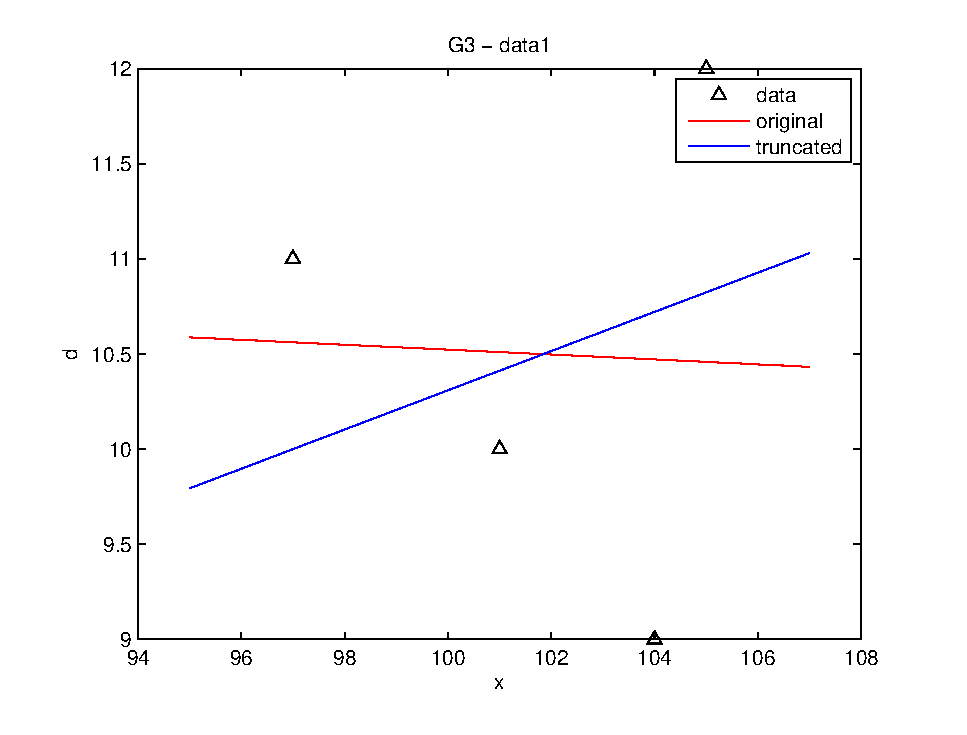
\includegraphics[width=12cm]{p2fig3.eps}
  \end{center}
\end{figure}
  \begin{figure}
\begin{center}
  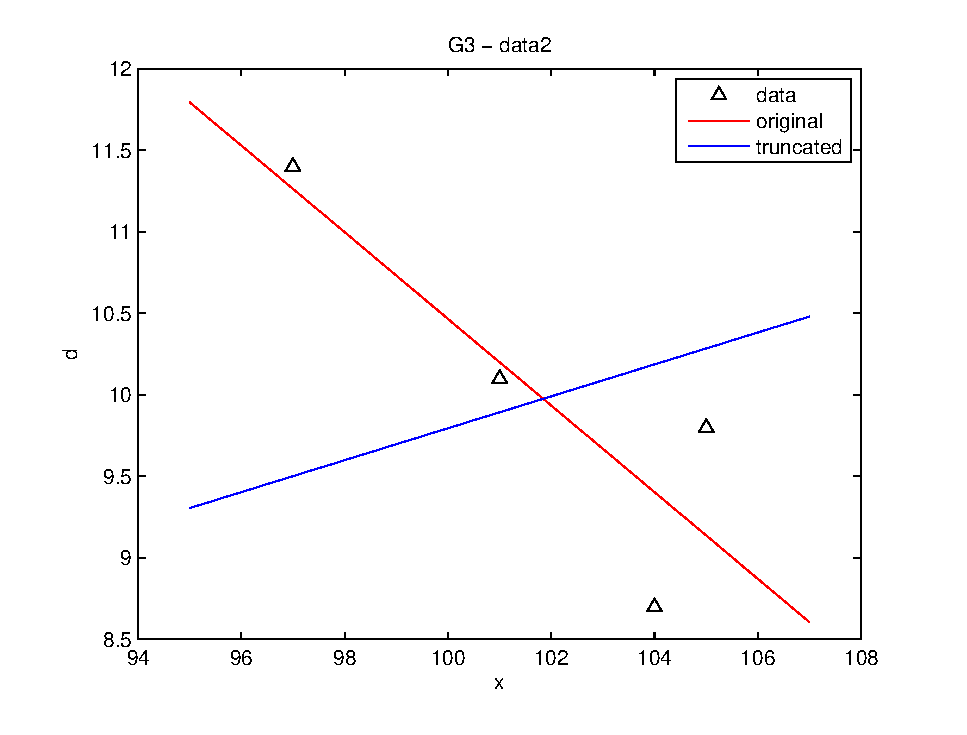
\includegraphics[width=12cm]{p2fig4.eps}
  \end{center}
\end{figure}

\subsubsection*{(e)- 5 points}
Looking at the plots we can see a large difference between the original and the truncated cases.  We have truncated the smallest singular value, which influences both rows of the generalized inverse.  However, it more significantly influences the first row, which controls our model parameter $m_1$ (the y-intercept).  If we look at our original models, most seem to fit the data reasonably (as reasonably as a line can fit) and all have a negative slope.  Our truncated models all have positive slopes and many don't seem to explain the data well at all.  This is because our truncation eliminated any information about y-intercept, and thus all the models have y-intercepts of 0 no matter what the data.  We can see this behavior clearly on the y-intercept on Toby's plots in the solution for problem 3.  As far as which models we would prefer, it would depend on what we know about the dataset.  In all cases besides G3-data 1 we would likely prefer the original models because they seem to fit the data better, unless we had some prior information about the y-intercept.  For the G3-data 1 neither model seems to fit very well, so it may be better to prefer the truncated model as it is more likely to avoid errors.


\subsection*{Problem 3 (graded by Toby) 20 points}

\subsubsection*{(a)- 5 points}
The MATLAB code that generates the matrices is attached at the end of this section. The matrices are calculated using $\v{m} = (\v{G}^T\v{G} + \alpha^2 \v{1})^{-1} \v{G}^T \v{d}$.
The matrices are
\begin{subequations}
\begin{align}
\nonumber\v{G}_{1,g,T,\alpha_1}^{-1} &= 
\begin{pmatrix} 
0.282931351378109  & 0.462937664456661 &  0.147926616569195 & 0.102925038299558\\
-0.019222102718031 & -0.122340004924458  & 0.058116323936789 & 0.083895799488396   
\end{pmatrix}\\
\nonumber\v{G}_{2,g,T,\alpha_1}^{-1} &= 
\begin{pmatrix}
   0.275661587810746 &  0.215517241379310 &  0.320769847634322 &  0.185445068163593\\
  -0.351343223736969 &  0.452586206896552 & -0.954290296712109 &  0.854550922213312
\end{pmatrix}\\
\nonumber\v{G}_{3,g,T,\alpha_1}^{-1} &= 
\begin{pmatrix}
   0.604003054340609  & 3.462399532543330  &-1.539794304311428 & -2.254393423862098\\
  -0.003493985867091 & -0.031656565418916 &  0.017627948796778 &  0.024668593684735
\end{pmatrix}\\
\nonumber\v{G}_{4,g,T,\alpha_1}^{-1} &= 
\begin{pmatrix}
   0.024993751562093 &  0.024993751562093 &  0.024993751562093  & 0.024993751562093\\
   0.074981254686328  & 0.074981254686328 &  0.074981254686328 &  0.074981254686328
\end{pmatrix}\\
\nonumber\v{G}_{3,g,T,\alpha_1}^{-1} &= 
\begin{pmatrix}
   0.262125138837468  & 0.427989633469086  & 0.137726767863754  & 0.096260644205850\\
  -0.016290262865605 & -0.116993706034802 &  0.059237319511292 &  0.084413180303591
\end{pmatrix}\\
\nonumber\v{G}_{3,g,T,\alpha_2}^{-1} &= 
\begin{pmatrix}
   0.251592356687898  & 0.213375796178344 &  0.280254777070064 &  0.194267515923567\\
  -0.230891719745223  & 0.310509554140127 & -0.636942675159236 &  0.581210191082802
\end{pmatrix}\\
\nonumber\v{G}_{4,g,T,\alpha_1}^{-1} &= 
\begin{pmatrix}
   0.032727078270480  & 0.187497400490787 & -0.083350663394751 & -0.122043243949828\\
   0.002115257782188 &  0.000499105768831 &  0.003327371792206  & 0.003731409795545
\end{pmatrix}\\
\nonumber\v{G}_{4,g,T,\alpha_2}^{-1} &= 
\begin{pmatrix}
   0.024844720496894 &  0.024844720496894  & 0.024844720496894  & 0.024844720496894\\
   0.074534161490683  & 0.074534161490683 &  0.074534161490683  & 0.074534161490683
\end{pmatrix}
\end{align}
\end{subequations}

\subsubsection*{(b)- 5 points}

For the generalized inverse we have that
\begin{equation}
\v{G}_g^{-1} = \sum_{i=1}^p \frac{s_i^2}{s_i^2+\alpha^2}\frac{1}{s_i}\v{v}_i
\v{u}_i^T,
\end{equation}
where $p$ is the index of the last nonzero singular value. For the regularized inverse, we have extra factors in the expansion that introduce a ``smooth'' truncation, i.e., for large $s_i$ the term is 1 and for small $s_i$ it is zero. This means that the similarity between the truncated and regularized matrices is determined by the relative size of the singular values compared to $\alpha$. For $\v{G}_1$, $\v{G}_2$ the singular values are larger than the Tikhonov parameters, implying that the truncated and regularized inverses should look different. For $\v{G}_3$ we have that $s_1^2 >> \alpha_1^2, \alpha_2^2$, $s_2^2 \sim \alpha_1^2$ and $s_2^2 << \alpha_2^2$. According to the equation above, this implies that the truncated and regularized inverses are different for $\alpha=0.1$, but similar for $\alpha=0.5$. For $\v{G}_4$ the truncated and the regularized must be different, because we only have two singular values, one of which is $0$ anyway.

\subsubsection*{(c)- 5 points}
The four plots are

\noindent Here is a plot of the profile:
\begin{figure}
\begin{center}
  \includegraphics[width=12cm]{p3b1.eps}
  \end{center}
\end{figure}
\begin{figure}
\begin{center}
  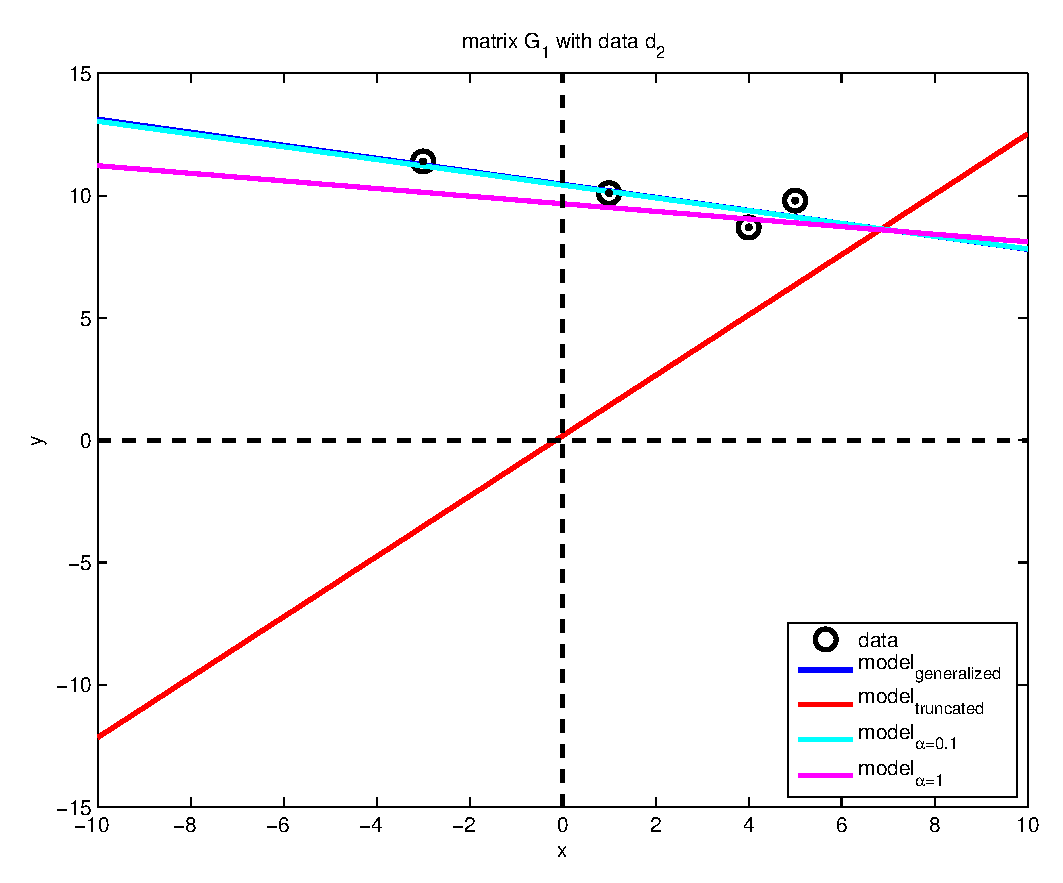
\includegraphics[width=12cm]{p3b2.eps}
  \end{center}
\end{figure}
\begin{figure}
\begin{center}
  \includegraphics[width=12cm]{p3b3.eps}
  \end{center}
\end{figure}
\begin{figure}
\begin{center}
  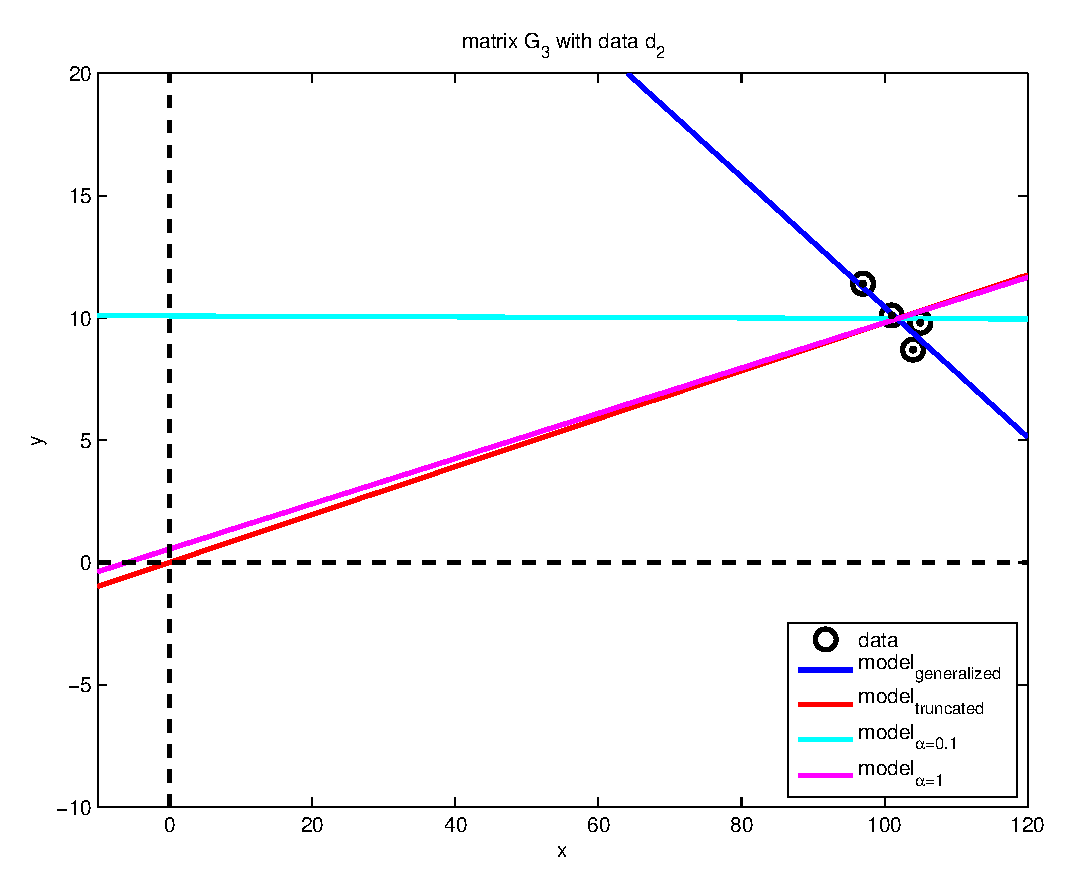
\includegraphics[width=12cm]{p3b4.eps}
  \end{center}
\end{figure}

\subsubsection*{(d)- 5 points}

For $\v{G}_3$ the truncated model and the Tikhonov model with $\alpha=0.5$ are very close. This is because of a term $s_i^2/(s_i^2+\alpha^2)$ in the expansision for the generalized inverse in terms of its singular values is almost zero for the smallest singular value of $G_3$ and almost $1$ for the largest singular value when $\alpha = 0.5$. Thus the truncated and the regularized models are very close. 
This is not the case for $\v{G}_1$, because the singular values are not as far apart and always larger than $\alpha$, but not by several orders of magnitude. Thus the truncated and the regularized models are giving different answers. In fact, for small truncation parameters, the regurlazied model is close to the generalized inverse model.

\noindent MATLAB script:
\lstinputlisting{p3.m}


\end{document}
